\chapter{The Ladder on Counts and Kingman's Coalescent}\label{ch:counts}\index{latent count}\index{coalescence}\index{complete monotonicity}

Chapter~\ref{ch:strong} built the Migdal Kadanoff ladder and its projected form, and left open what the exact ladder, without the projection, does to a link density. The heat kernel and the Wilson law are mixtures $\E[(1+\cos\theta)^{M_0}]$ over a random nonnegative integer $M_0$ (Corollary~\ref{cor:Mclosed} below; Section~\ref{ch:langlands} of the later Chapter~\ref{ch:kacyang} returns to this reading). Bond moving adds such counts, and this chapter proves that decimation thins them by a positive kernel. The exact Migdal Kadanoff ladder for SU(2), with no projection, is then a map on the laws of a nonnegative integer, and we can look at it.

\section{The coalescence theorem}

Write $x=\cos\theta$, let $C_n$ be the Catalan numbers, and let
\[
f_j(x)=\frac{2^j}{C_{j+1}}\,(1+x)^j,\qquad j=0,1,2,\dots
\]
be the probability densities with respect to Haar measure. Convolution is on the group.

\begin{theorem}[coalescence]\label{thm:coalescence}
For all integers $a,b\ge0$,
\[
f_a*f_b=\sum_{j=0}^{\min(a,b)}Q(j\mid a,b)\,f_j ,
\]
where $Q(\cdot\mid a,b)$ is a probability law on $\{0,\dots,\min(a,b)\}$ with every weight strictly positive, and
\[
\sum_jj\,Q(j\mid a,b)=\frac{ab}{a+b+2}.
\]
\end{theorem}

The proof has three steps, each elementary.

\begin{lemma}[characters of $f_j$]\label{lem:fjchar}
With $J=j+1$, $f_j=\sum_{n=1}^{J}n\,u_n(J)\,\chi_n$ where
\[
u_n(J)=\frac{(J-1)!\,(J+1)!}{(J-n)!\,(J+n)!}=\frac{J+1}{J}\,\binom{2J}{J-n}\Big/\binom{2J}{J}.
\]
\end{lemma}

\begin{proof}
$2+2\cos\theta=(e^{i\theta/2}+e^{-i\theta/2})^2$, so $(2+2x)^j=\sum_m\binom{2j}{j-m}e^{im\theta}$, and collecting $e^{im\theta}$ into characters $\chi_n=\sum_{|m|<n,\ m\equiv n-1}e^{im\theta}$ gives the coefficient $\binom{2j}{j-n+1}-\binom{2j}{j-n-1}=2n\,(2j+1)!/\big((j-n+1)!\,(j+n+1)!\big)$ of $\chi_n$. Normalise by the coefficient of $\chi_1$.
\end{proof}

So the fundamental coefficient is $u_2=(J-1)/(J+2)=j/(j+3)$, as in Proposition~\ref{prop:latentcount}, and as a function of $n$ the sequence $u_n(J)$ is, up to a constant, the law of the endpoint of a simple random walk of $2J$ steps.

\begin{lemma}[a completely monotone function]\label{lem:cm}
For an integer $N\ge1$ let $w_N(s)=1\big/\big(\Gamma(N+1-\sqrt s)\,\Gamma(N+1+\sqrt s)\big)$. Then
\[
w_N(s)=\frac1{(N!)^2}\prod_{i>N}\Big(1-\frac s{i^2}\Big),
\]
and $(-1)^kw_N^{(k)}(s)>0$ for all $k\ge0$ and $0\le s<(N+1)^2$.
\end{lemma}

\begin{proof}
The product formula follows from $\Gamma(1+z)\Gamma(1-z)=\pi z/\sin\pi z$ and Euler's product for the sine. Each factor is positive, linear and decreasing on $[0,(N+1)^2)$; a finite product of such functions has derivatives of alternating sign by Leibniz's rule, and the signs pass to the limit, which is uniform on compact subsets together with all derivatives.
\end{proof}

\begin{proof}[Proof of Theorem~\ref{thm:coalescence}]
Convolution multiplies the coefficients $u_n$. Put $\bar a=a+1\le \bar b=b+1$ and $g_J(n)=1/\big((J-n)!\,(J+n)!\big)$, so that $u_n(J)=(J-1)!\,(J+1)!\,g_J(n)$. We must write $g_{\bar a}(n)\,g_{\bar b}(n)$, for $n=1,\dots,\bar a$, as a combination of $g_J(n)$, $J=1,\dots,\bar a$, with positive coefficients.

For $J\le \bar a$, $g_J(n)=g_{\bar a}(n)\,P_J(n^2)$ with $P_J(s)=\prod_{i=J+1}^{\bar a}(i^2-s)$, a polynomial of degree $\bar a-J$ that vanishes at $s=n^2$ for $J<n\le \bar a$, as $g_J(n)$ does. And $g_{\bar b}(n)=w_{\bar b}(n^2)$. So it is enough to find $\omega_J$ with
\[
w_{\bar b}(s)=\sum_{J=1}^{\bar a}\omega_J\,P_J(s)\qquad\text{at the nodes }s=1,4,\dots,\bar a^2 .
\]
This is Newton's interpolation formula with the nodes taken in the order $\bar a^2,(\bar a-1)^2,\dots,1$: the basis polynomials are $\prod_{i<k}(s-s_i)=(-1)^kP_{\bar a-k}(s)$, so
\[
\omega_{\bar a-k}=(-1)^k\,w_{\bar b}\big[\bar a^2,(\bar a-1)^2,\dots,(\bar a-k)^2\big],
\]
a divided difference. By the mean value theorem for divided differences it equals $(-1)^kw_{\bar b}^{(k)}(\xi)/k!$ for some $\xi\in[1,\bar a^2]$, which is positive by Lemma~\ref{lem:cm} because $\bar a\le \bar b$. Hence
\[
Q(j\mid a,b)=\omega_J\,\frac{(\bar a-1)!\,(\bar a+1)!\,(\bar b-1)!\,(\bar b+1)!}{(J-1)!\,(J+1)!}>0,\qquad J=j+1 .
\]
The weights sum to one because $u_1=1$ on both sides.

For the mean, use the functional $\mathsf W(f)=\int f(x)\,(1-x)^{-1}$ against Haar measure. Since $\int\chi_n(1-x)^{-1}=\frac2\pi\int_0^\pi\sin n\theta\cot\frac\theta2\,d\theta=2$ for every $n$, $\mathsf W(f)=2\sum_nn\,u_n$. On $f_j$, where $\cos^2(\theta/2)$ is Beta with parameters $j+\frac32,\frac32$, it equals $j+2$. So the mean of $j+2$ under $Q$ is $2\sum_nn\,u_n(\bar a)u_n(\bar b)$. With $d_n=\binom{2\bar a}{\bar a-n}\binom{2\bar b}{\bar b-n}$ one checks $(\bar a+n)(\bar b+n)\,d_n-(\bar a+n+1)(\bar b+n+1)\,d_{n+1}=2n(\bar a+\bar b)\,d_n$, so the sum telescopes:
\[
\sum_{n\ge1}n\,d_n=\frac{(\bar a+1)(\bar b+1)}{2(\bar a+\bar b)}\,d_1,
\]
hence
\[
2\sum_{n\ge1}n\,u_n(\bar a)u_n(\bar b)=\frac{(\bar a+1)(\bar b+1)}{\bar a+\bar b},
\]
and $\frac{(\bar a+1)(\bar b+1)}{\bar a+\bar b}-2=\frac{(\bar a-1)(\bar b-1)}{\bar a+\bar b}=\frac{ab}{a+b+2}$.
\end{proof}

Two small cases: $Q(\cdot\mid1,b)=\big(\frac3{b+3},\frac b{b+3}\big)$ and $Q(\cdot\mid3,3)=\big(\frac5{28},\frac{15}{28},\frac{15}{56},\frac1{56}\big)$. The script \texttt{count\_ladder.py} computes $Q$ in rational arithmetic and confirms positivity and the mean for all $a\le b\le20$; the theorem makes that check redundant, and it was the check that suggested the theorem.

\section{The kernel is hypergeometric}\label{sec:hypergeometric}\index{hypergeometric distribution}\index{Chu Vandermonde identity}

The Newton formula of the last proof hides a closed form. It was found by looking at the numerators of $Q(\cdot\mid3,3)=\frac1{56}(10,30,15,1)$.

\begin{theorem}[the coalescence is an intersection]\label{thm:hypergeometric}
For all $a,b\ge0$ and $0\le j\le\min(a,b)$,
\[
Q(j\mid a,b)=\binom aj\binom{b+2}{b-j}\Big/\binom{a+b+2}{b}.
\]
This is the hypergeometric law: $Q(\cdot\mid a,b)$ is the law of the number of common elements of two independent uniformly random subsets, of sizes $a$ and $b$, of a set of size $a+b+2$.
\end{theorem}

\begin{proof}
We must show $\sum_jQ(j\mid a,b)\,u_n(j+1)=u_n(a+1)\,u_n(b+1)$ for every $n$, with $u_n(j+1)=j!\,(j+2)!/\big((j+1-n)!\,(j+1+n)!\big)$. Substituting, and putting $j=n-1+i$, $a'=a-n+1$, $b'=b-n+1$,
\[
\sum_j\binom aj\binom{b+2}{j+2}u_n(j+1)=\frac{a!\,(b+2)!}{a'!\,b'!\,(2n)!}\sum_{i\ge0}\frac{(-a')_i(-b')_i}{i!\,(2n+1)_i},
\]
and the sum on the right equals
\[
\frac{(a+b+2)!\,(2n)!}{(a+n+1)!\,(b+n+1)!}
\]
by the Chu Vandermonde identity ${}_2F_1(-a',-b';c;1)=(c+b')_{a'}/(c)_{a'}$ with $c=2n+1$. The right side equals $\binom{a+b+2}{b}u_n(a+1)u_n(b+1)$.
\end{proof}

So the theorem of the first section is the Chu Vandermonde identity, and its positivity is the positivity of binomial coefficients. Everything observed about $Q$ now follows at once, and more.

\begin{corollary}\label{cor:hypergeometric}
\begin{enumerate}
\item[(i)] The mean of $Q(\cdot\mid a,b)$ is $ab/(a+b+2)$ and its variance is
\[
\frac{ab\,(a+2)(b+2)}{(a+b+2)^2(a+b+1)} .
\]
\item[(ii)] $Q(j\mid a,b)$ is totally positive of order two in $(j,a)$ for each $b$ and in $(j,b)$ for each $a$. This settles Open problem~\ref{op:Qtp2}.
\item[(iii)] Without normalisation,
\[
(1+x)^a*(1+x)^b=c(a,b)\sum_{j=0}^{\min(a,b)}\frac{2^{j-1}\,(1+x)^j}{(2j+1)!\,(a-j)!\,(b-j)!},
\]
where
\[
c(a,b)=\frac{(2a+2)!\,(2b+2)!}{2^{a+b}(a+1)(b+1)\,(a+b+2)!} .
\]
\item[(iv)] For the death process $A$ of Section~\ref{ch:kingman}, $P_a\big(A(\tau)=j\big)=\sum_bP_\infty\big(A(\tau)=b\big)\,Q(j\mid a,b)$: the lineages left at time $\tau$ from $a$ are the intersection of the $a$ with an independent sample from the entrance law.
\end{enumerate}
\end{corollary}

\begin{proof}
(i) is the mean and variance of the hypergeometric law with population $a+b+2$, $a$ marked elements and $b$ draws. (ii): $\binom aj$ is totally positive in $(a,j)$ and $\binom{b+2}{b-j}=(b+2)!/\big((b-j)!\,(j+2)!\big)$ is totally positive in $(b,j)$, because $1/k!$ is log concave; every other factor is a function of $j$ alone or of $(a,b)$ alone. (iii) follows from the theorem and $\int(1+x)^m=C_{m+1}2^{-m}$. (iv) is Theorem~\ref{thm:kingman} written with $K_s=\sum_b\pi_s(b)f_b$, $\pi_s(b)=P_\infty\big(A(s/2)=b\big)$.
\end{proof}

\paragraph{\normalfont\scshape The exact ladder as an urn.} The exact Migdal Kadanoff ladder for SU(2) is now a scheme that could be explained to a student of elementary probability. A link carries a random finite set, whose size has the law $\nu_0$. To move bonds, take the disjoint union of $k$ independent copies. To decimate, reweight sizes by $C_{m+1}2^{-m}$, take two independent sets of sizes $a$ and $b$, throw them uniformly at random into a universe of $a+b+2$ points, keep the intersection, and repeat. In flat space the universe would have $a+b$ points, and the mean size of the intersection would be the harmonic rule $ab/(a+b)$. The two extra points are the curvature of the group. They are the same $2$ as in the death rate $\frac12m(m+2)$ of Kingman's process with mutation~\cite{Gri80,Tav84} and as in $\theta_{\mathrm m}-1$ for the mutation parameter $\theta_{\mathrm m}=3$, the dimension of the group.

\paragraph{\normalfont\scshape The drift, explained.} Open problem~\ref{op:drift} asked why the mean count falls by one half at each rung. With an explicit kernel the first two moments can be followed. Let $m$ and $v$ be the mean and variance of the count and $r=v/m$. For large $m$, by the delta method:
\begin{itemize}
\item bond moving with $k=4$ multiplies the variance by $4$ and sends the mean to $4m+\frac92r$, the correction coming from the weights $C_{j+1}2^{-j}\sim2^jj^{-3/2}$, which are removed before the counts are added and restored after;
\item one coalescence of two independent counts of mean $M$ and variance $V$ has mean $\frac M2-\frac12-\frac V{4M}$ and variance $\frac M8+\frac V8$, by Corollary~\ref{cor:hypergeometric}(i).
\end{itemize}
Two coalescences after one bond moving give
\[
m'=m-\frac{13}{16}+\frac{15}{16}\,r+O\Big(\frac1m\Big),\qquad r'=\frac5{16}+\frac r{16}+O\Big(\frac1m\Big).
\]
The ratio $r$ converges geometrically, with factor $\frac1{16}$, to $r_*=\frac13$, and at $r_*$ the drift is $-\frac{13}{16}+\frac5{16}=-\frac12$. The fixed ratio $\frac13$ is that of Kingman's coalescent coming down from infinity, so the heat kernel has it from the start.

\begin{table}[t]
\centering\small
\begin{tabular}{lcccc}
\toprule
starting law & mean count & $r$ & predicted drift & exact drift \\ \midrule
point mass at $60$ & 60.0 & 0 & $-0.8125$ & $-0.8075$ \\
heat kernel, $\beta=4$ & 6.87 & 0.388 & $-0.448$ & $-0.507$ \\
heat kernel, $\beta=16$ & 30.8 & 0.346 & $-0.488$ & $-0.502$ \\
Wilson, $\kappa=32$ & 62.5 & 1.024 & $+0.147$ & $+0.118$ \\
\bottomrule
\end{tabular}
\caption[The drift, predicted and exact]{The change of the mean count over one exact rung ($k=4$, $\ell^2=4$) from four starting laws: the prediction $-\frac{13}{16}+\frac{15}{16}r$ from the delta method, with $r$ the ratio of variance to mean of the starting count, against the exact value.}
\label{tab:drift}
\end{table}

\begin{figure}[t]
\centering
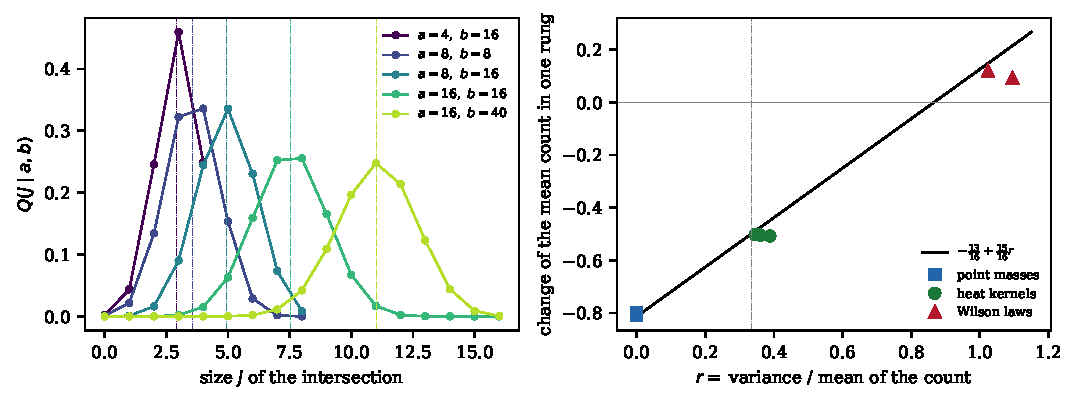
\includegraphics[width=\textwidth]{figures/counts_urn.pdf}
\caption[The hypergeometric kernel and the drift law]{Left: the coalescence kernel $Q(j\mid a,b)$, the hypergeometric law of the intersection of two random subsets of sizes $a$ and $b$ in a set of size $a+b+2$; dotted lines mark the means $ab/(a+b+2)$. Right: the change of the mean count over one exact rung against the ratio $r$ of variance to mean, for point masses, heat kernels and Wilson laws, with the line $-\frac{13}{16}+\frac{15}{16}r$; the vertical line is the fixed ratio $\frac13$.}
\label{fig:countsurn}
\end{figure}

The three numbers that had no explanation, a drift of $-0.81$ from a point mass, $-0.51$ from a heat kernel and $+0.11$ from a Wilson law, are $-\frac{13}{16}$, $-\frac12$ and $+\frac18$ (the first and third are proved in Theorem~\ref{thm:firstrung}, the second is not), the values of one linear function at $r=0$, $\frac13$ and $1$; the residual differences in Table~\ref{tab:drift} are the corrections of order $1/m$. A Wilson law has a Poisson count, with $r=1$, which is above the threshold $r=\frac{13}{15}$ at which the drift changes sign. That is why it gains order at its first rung. After one rung its ratio is $\frac38$ and its drift $-0.46$, after two $\frac13$ to within one percent. So the transient of Table~\ref{tab:notmonotone} (in Section~\ref{ch:kingman} below) lasts one rung, and the invariant class we were looking for is, to this order, a neighbourhood of the ray $r=\frac13$. The derivation is an asymptotic calculation and not a theorem; the kernel it rests on is exact.

\section{Consequences}

\begin{corollary}[the family $\mathcal M$ is closed]\label{cor:Mclosed}
Let $\mathcal M$ be the set of densities $\sum_j\pi(j)f_j$ with $\pi$ a probability law on the nonnegative integers. Then $\mathcal M$ contains every SU(2) heat kernel and every Wilson law, and is closed under products followed by normalisation and under convolution. Hence every rung of the exact Migdal Kadanoff ladder started from a heat kernel or a Wilson law, for any integer scale factor and any dimension, lies in $\mathcal M$. (Products are taken of bounded densities, so that the normalisation is finite; heat kernels and Wilson laws are bounded, and bounded densities stay bounded under products and convolutions.)
\end{corollary}

\begin{proof}
The Wilson law has density proportional to $e^{\kappa x}=e^{-\kappa}\sum_{m\ge0}\kappa^m(1+x)^m/m!$, a series of positive multiples of $f_m=2^mC_{m+1}^{-1}(1+x)^m$, so it lies in $\mathcal M$. The heat kernel lies in $\mathcal M$ by Theorem~\ref{thm:kingman}(ii), whose proof uses only Lemma~\ref{lem:fjchar}. For products, $f_af_b=\big(2^{a+b}/C_{a+1}C_{b+1}\big)(1+x)^{a+b}$ is a positive multiple of $f_{a+b}$, so if $\rho=\sum_a\pi(a)f_a$ and $\sigma=\sum_b\pi'(b)f_b$ then $\rho\sigma=\sum_{a,b}\pi(a)\pi'(b)\,c_{ab}f_{a+b}$ with $c_{ab}>0$ (all terms are nonnegative, so the double series may be rearranged); when $\rho\sigma$ is integrable, its normalisation is a probability density of the same form (and $\int\rho\sigma>0$, since every $f_j$ is positive off the antipode). For convolution, Theorem~\ref{thm:coalescence} and the same rearrangement give $\rho*\sigma=\sum_{a,b}\pi(a)\pi'(b)\sum_jQ(j\mid a,b)f_j=\sum_j\pi''(j)f_j$ with $\pi''(j)=\sum_{a,b}\pi(a)\pi'(b)Q(j\mid a,b)\ge0$, and $\sum_j\pi''(j)=1$ because each $Q(\cdot\mid a,b)$ is a probability law. Finally one rung with integer scale factor $\ell$ in dimension $d$ is the normalised power $\rho^{\ell^{d-2}}$ (bond moving) followed by the $\ell^2$ fold convolution (decimation), which are repeated products and convolutions with integer multiplicities; bounded densities stay bounded, as $\|\rho*\sigma\|_\infty\le\|\rho\|_\infty$.
\end{proof}

So at every rung of the exact ladder the density of a link is an absolutely monotone function of $1+\cos\theta$: all of its derivatives in $\cos\theta$ are nonnegative. In particular it is increasing and convex in $\cos\theta$, its character coefficients are positive, and it is a mixture of functions of positive type. None of this was known to us for the exact ladder before; the projection onto heat kernels had hidden it.

\begin{corollary}[the mean count is an observable]\label{cor:meancount}
For $\rho=\sum_j\pi(j)f_j$ in $\mathcal M$,
\[
\sum_jj\,\pi(j)=\Big\langle\frac1{1-\cos\theta}\Big\rangle_\rho-2=2\sum_{n\ge1}n\,u_n(\rho)-2 .
\]
For the heat kernel this is $2\sum_nn\,e^{-(n^2-1)t/4}-2=2\beta-\frac76+O(1/\beta)$.
\end{corollary}

\begin{proof}
The first equality is Proposition~\ref{prop:observable}, whose proof is by linearity from $\rho=f_j$, together with $\int\chi_n(1-\cos\theta)^{-1}=2$. For the heat kernel, $u_n=e^{-(n^2-1)t/4}$ with $t=2/\beta$, and the first Euler Maclaurin sum in the proof of Theorem~\ref{thm:harmonic} with $H_1=t/4=1/(2\beta)$ gives $2e^{H_1}\big(\frac1{2H_1}-\frac1{12}\big)-2=2\beta-\frac76+O(1/\beta)$.
\end{proof}

\paragraph{\normalfont\scshape The two operations.} Let $\nu_0$ be the law of $M_0$ in $\rho\propto\E[(1+x)^{M_0}]$, so that $\pi(j)\propto\nu_0(j)\,C_{j+1}2^{-j}$. Then bond moving with power $k$ and one convolution of decimation act by
\[
\nu_0\ \longmapsto\ \nu_0^{*k}\qquad\text{and}\qquad\pi\ \longmapsto\ \sum_{a,b}\pi(a)\,\pi(b)\,Q(\cdot\mid a,b),
\]
the first being the law of the sum of $k$ independent counts. The first multiplies the mean of $M_0$ by $k$. The second sends two counts $a$ and $b$ to a count of mean $ab/(a+b+2)$, which is less than the flat value $ab/(a+b)$ and less than $\min(a,b)$. A population is multiplied, then thinned in pairs. In flat space the thinning would exactly undo the multiplication in four dimensions; the $2$ in the denominator is what is left over, and it is the curvature of the group once more.

\paragraph{\normalfont\scshape Random walks.} By Lemma~\ref{lem:fjchar} the theorem is a statement about simple random walk: the pointwise product of the endpoint laws of two walks of $2\bar a$ and $2\bar b$ steps, restricted to $n\ge1$, is a positive combination of the endpoint laws of walks of $2J$ steps with $J\le\min(\bar a,\bar b)$. Two walks conditioned to end together look, at their common endpoint, like one shorter walk of random length. We have not found this statement in the literature; it may well be there.

\paragraph{\normalfont\scshape A worked case.} Take $a=b=2$, so $\bar a=\bar b=3$. The nodes are $s=9,4,1$ and $w_3(n^2)=1/\big((3-n)!\,(3+n)!\big)$ gives $w_3(9)=\frac1{720}$, $w_3(4)=\frac1{120}$, $w_3(1)=\frac1{48}$. The divided differences are
\[
w_3[9]=\tfrac1{720},\qquad w_3[9,4]=-\tfrac1{720},\qquad w_3[9,4,1]=\tfrac1{2880},
\]
alternating in sign as Lemma~\ref{lem:cm} requires, so $\omega_3=\frac1{720}$, $\omega_2=\frac1{720}$, $\omega_1=\frac1{2880}$. Multiplying by $(2!\,4!)^2/\big((J-1)!\,(J+1)!\big)$, which is $48$, $384$ and $1152$ for $J=3,2,1$, gives $Q(2)=\frac1{15}$, $Q(1)=\frac8{15}$, $Q(0)=\frac25$, with mean $\frac23=\frac{2\cdot2}{2+2+2}$.

\section{The exact ladder, looked at}

With the theorem in hand the exact ladder can be run on counts with no quadrature on the group: add four independent copies of $M_0$, reweight, and apply the coalescence twice. Starting from heat kernels at $\beta=2$, $3$ and $4$, with $k=4$ and $\ell^2=4$, where $\ell=2$ is the Migdal Kadanoff scale factor, written $b$ in Chapter~\ref{ch:strong}, in Table~\ref{tab:rungs}:

\begin{table}[t]
\centering\footnotesize
\begin{tabular}{lcccccccc}
\toprule
rung & 0 & 1 & 2 & 3 & 4 & 5 & 6 & 7 \\ \midrule
count, $\beta=4$ & 6.874 & 6.366 & 5.860 & 5.352 & 4.845 & 4.337 & 3.829 & 3.321 \\
$u_2$, $\beta=4$ & 0.687 & 0.670 & 0.651 & 0.629 & 0.604 & 0.576 & 0.544 & 0.507 \\
count, $\beta=3$ & 4.888 & 4.379 & 3.871 & 3.363 & 2.854 & & & \\
count, $\beta=2$ & 2.916 & 2.407 & 1.899 & 1.394 & 0.896 & & & \\
\bottomrule
\end{tabular}
\caption[The exact ladder on counts, by rung]{The mean count and the fundamental coefficient $u_2$ at each rung of the exact ladder ($k=4$, $\ell^2=4$), labelled by the starting heat kernel coupling $\beta$.}
\label{tab:rungs}
\end{table}

\begin{figure}[t]
\centering
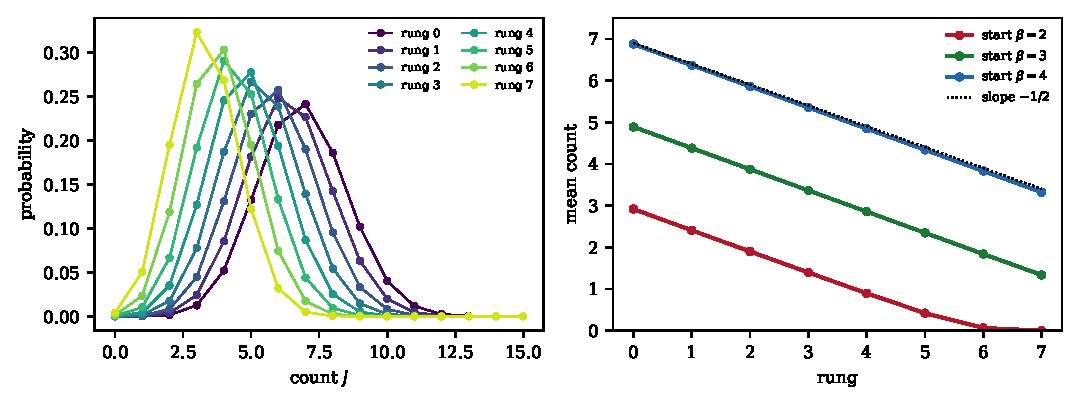
\includegraphics[width=\textwidth]{figures/counts.pdf}
\caption[The exact ladder on counts]{The exact Migdal Kadanoff ladder for SU(2), $\ell=2$ in four dimensions, as a process on integer counts. Left: the law of the count at eight successive rungs, started from the heat kernel at $\beta=4$. Right: the mean count against the rung from three starting couplings, with a line of slope $-\frac12$.}
\label{fig:counts}
\end{figure}

Three observations, the first two numerical and the third now partly a theorem.

The mean count falls by very nearly one half at each rung: $0.508$, $0.506$, $0.508$, $0.507$, $0.508$, $0.508$, $0.508$ from $\beta=4$, and the same from the other starts until the count is of order one (Figure~\ref{fig:counts}). In the count the exact ladder is a walk with constant drift. Since the mean count is $2\beta-\frac76$ to leading order, this is the decrement $\frac14$ of Theorem~\ref{thm:expansion}, now seen for the exact ladder and holding far outside weak coupling. The observable that falls linearly is $\langle1/(1-\cos\theta)\rangle$.

Along the computed heat kernel orbits the law of the count at each rung is below the law at the previous rung in the likelihood ratio order, and the law $\nu_0$ is log concave at every rung. So the exact ladder is monotone along these orbits in the strongest order available, and $u_2=\E[j/(j+3)]$ decreases.

The kernel $Q(j\mid a,b)$ is totally positive of order two in $(j,a)$ for each fixed $b$, and stochastically increasing in $a$, for all $a,b\le20$, in exact arithmetic (the total positivity is Corollary~\ref{cor:hypergeometric}(ii)). It is not totally positive in $(a,b)$ for fixed $j$, and should not be: the two parents compete.

\section{The harmonic law}\label{sec:harmonic}\index{harmonic law}

The drift law of Section~\ref{sec:hypergeometric} was obtained by the delta method. For decimation it can be made a theorem, because the mean count is linear in the law and the characters of the $f_j$ are explicit. Write $J=j+1$, so that $u_n(J)=\prod_{i=1}^{n-1}(J-i)/(J+1+i)$, and for $J_1,\dots,J_p$ put
\[
H_1=\sum_i\frac1{J_i},\qquad H_2=\sum_i\frac1{J_i^2},\qquad H_3=\sum_i\frac1{J_i^3}.
\]

\begin{theorem}[the harmonic law]\label{thm:harmonic}
Fix $p\ge2$ and $\lambda\ge1$. For $J_1,\dots,J_p$ with $\max J_i\le\lambda\min J_i$, the mean count of $f_{J_1-1}*\cdots*f_{J_p-1}$ is
\[
\frac1{H_1}-\frac76+\frac{H_2}{2H_1^2}-\frac{H_3}{3H_1^3}+R,\qquad |R|\le\frac{c(p,\lambda)}{\min J_i}.
\]
\end{theorem}

\begin{proof}
The mean count of a law with character coefficients $u_n$ is $2\sum_nn\,u_n-2$, and those of the convolution are $\prod_iu_n(J_i)$. Three facts about $u_n(J)$ are needed. First, since $\log(1-x)\le-x$ and $\log(1+y)\ge y/2$ for $0\le y\le1$, and $u_n(J)=0$ for $n>J$,
\[
u_n(J)\le\exp\Big(-\sum_{i=1}^{n-1}\frac{2i+1}{2J}\Big)=e^{-(n^2-1)/(2J)}.
\]
Second, expanding the logarithms to third order and summing over $i$,
\[
\log u_n(J)=-\frac{n^2-1}{J}+\frac{n^2-1}{2J^2}-\frac{n^4}{6J^3}+O\Big(\frac{n^2}{J^3}+\frac{n^4}{J^4}+\frac{n^6}{J^5}\Big),
\]
uniformly for $n\le J^{3/5}$. Third, by the Euler Maclaurin formula, as $H_1\to0$,
\[
\sum_{n\ge1}n\,e^{-H_1n^2}=\frac1{2H_1}-\frac1{12}+O(H_1),\qquad \sum_{n\ge1}n^3e^{-H_1n^2}=\frac1{2H_1^2}+O(1),
\]
\[
\sum_{n\ge1}n^5e^{-H_1n^2}=\frac1{H_1^3}+O(1).
\]
By the first fact the terms with $n>J^{3/5}$ contribute less than any power of $1/J$. For the others the second fact gives
\[
\prod_iu_n(J_i)=e^{H_1}e^{-H_1n^2}\Big(1+\frac{H_2n^2}{2}-\frac{H_3n^4}{6}+\varepsilon_n\Big),
\]
where $\sum_nn\,e^{-H_1n^2}|\varepsilon_n|=O(1/\min J_i)$, because each term of $\varepsilon_n$ is of relative order $J^{-2}$ when $n$ is of order $\sqrt J$ and the leading sum is of order $J$. The third fact then gives
\[
\sum_nn\prod_iu_n(J_i)=\Big(1+H_1\Big)\Big(\frac1{2H_1}-\frac1{12}\Big)+\frac{H_2}{4H_1^2}-\frac{H_3}{6H_1^3}+O\Big(\frac1{\min J_i}\Big),
\]
and doubling and subtracting $2$ gives the statement.
\end{proof}

The leading term is the harmonic sum: counts compose under decimation as resistances in parallel, or as $J=2\beta$ composes for heat kernels, where $1/J$ is proportional to time and times add. The constant $-\frac76$ is the one in Corollary~\ref{cor:meancount}. For $p=2$ the theorem can be compared with the exact mean $ab/(a+b+2)=1/H_1-1+1/(J_1+J_2)$: the three constants of the theorem sum to $-1$ for every ratio $J_1/J_2$, as they should.

\begin{corollary}[the drift from a point mass]\label{cor:pointdrift}
The exact rung with $k$ copies and $p$ fold convolution takes $f_m$ to a law with mean count
\[
\frac{km}{p}+c_p+O\Big(\frac1m\Big),\qquad c_p=\frac{3}{2p}-\frac76-\frac1{3p^2}.
\]
For $k=p=4$ the drift is $c_4=-\frac{13}{16}$, and for $k=p=2$ it is $c_2=-\frac12$.
\end{corollary}

\begin{proof}
Bond moving takes $f_m$ to $f_{km}$ exactly. Put $J_i=km+1$ in the theorem: $1/H_1=(km+1)/p$, $H_2/2H_1^2=1/2p$ and $H_3/3H_1^3=1/3p^2$.
\end{proof}

So the first of the three unexplained numbers is a theorem. In rational arithmetic the drift from $f_m$ at $k=p=4$ is $-0.79759$, $-0.80875$ and $-0.81156$ at $m=20$, $80$ and $320$, approaching $-\frac{13}{16}$ at the rate $0.30/m$. As $p\to\infty$ the constant $c_p$ tends to $-\frac76$: a long convolution of point masses is a heat kernel, and its mean count is $2\beta-\frac76$.

\begin{corollary}[decimation of a concentrated law]\label{cor:decdrift}
Let $\pi_M$ be laws on the counts with mean $M\to\infty$, variance $vM+o(M)$ and $E|a-M|^3=O(M^{3/2})$. Then the $p$ fold convolution of $\sum_a\pi_M(a)f_a$ with itself has mean count
\[
\frac Mp+c_p-\frac{(p-1)\,v}{p^2}+o(1).
\]
\end{corollary}

\begin{proof}
The mean count is the expectation of the function of Theorem~\ref{thm:harmonic} over independent $a_1,\dots,a_p$ from $\pi_M$. The event that some $a_i$ lies outside $[M/2,2M]$ has probability $O(M^{-3/2})$ and the mean count never exceeds $\min a_i$, so that event contributes $o(1)$. On its complement expand $1/H_1$ to second order about $J_i=M+1$: the pure second derivatives are $-2(p-1)/(p^3M)$, the mixed ones have expectation zero, and the third derivatives are $O(M^{-2})$ against third moments $O(M^{3/2})$. The terms in $H_2$ and $H_3$ are continuous and take their values at the centre.
\end{proof}

At $p=4$ the correction is $-\frac3{16}v$, which is what two coalescences gave in Section~\ref{sec:hypergeometric}.

\section{The count as an observable, and the first rung}\label{sec:observable}\index{mean count!as an observable}

The other half of a rung is bond moving, and for it a different description of the mean count is the useful one.

\begin{proposition}[the count is an observable]\label{prop:observable}
For every $\rho=\sum_j\pi(j)f_j$ in $\mathcal M$ with finite mean count,
\[
\sum_jj\,\pi(j)=E_\rho\Big[\frac{1}{1-\cos\theta}\Big]-2=E_\rho\Big[\frac1{2\sin^2(\theta/2)}\Big]-2 .
\]
\end{proposition}

\begin{proof}
Both sides are linear in $\rho$, so take $\rho=f_j$. Under $f_j$ the variable $y=\cos^2(\theta/2)$ has the $\mathrm{Beta}(j+\frac32,\frac32)$ law, and $1-\cos\theta=2(1-y)$. For a $\mathrm{Beta}(a,b)$ variable $E[1/(1-y)]=(a+b-1)/(b-1)$, which here is $2(j+2)$; half of it, less $2$, is $j$.
\end{proof}

The function $2\sin^2(\theta/2)$ is the one of the lemma of Section~\ref{ch:routeB}, met here on the group. The proposition says that the latent count, which was introduced as a mixing variable, has a mean that can be measured on a configuration: it is the expectation of the reciprocal of the Wilson action density, less two. The singularity at the identity is integrable against Haar measure, which vanishes there like $\theta^2$. It also gives the count of a law in closed form to the order needed. For $\rho=c\prod_m(1+x/\gamma_m)$ in the class $\mathcal L$ of Chapter~\ref{ch:zeros}, the densities $c\prod_m(1+x/\gamma_m)$ with $\gamma_m\ge1$ and $\sum_m1/\gamma_m<\infty$ together with their locally uniform limits, put
\[
\Sigma_1=\sum_m\frac1{\gamma_m+1},\qquad \Sigma_2=\sum_m\frac1{(\gamma_m+1)^2},\qquad r=1-\frac{2\Sigma_2}{\Sigma_1},
\]
so that $\Sigma_1$ and $-\Sigma_2$ are the first two derivatives of $\log\rho$ in $x$ at the identity, and $0\le r<1$.

\begin{lemma}[count of a law with real zeros]\label{lem:Lcount}
For $\rho\in\mathcal L$ the count law $\pi$ has, as $\Sigma_1\to\infty$ and uniformly in the zeros,
\[
\text{mean}=2\Sigma_1-\frac32\,r+O(\Sigma_1^{-1/2}),\qquad \text{variance}=2\Sigma_1\,r+O(\Sigma_1^{1/2}),
\]
\[
E_\pi|j-2\Sigma_1|^3=O(\Sigma_1^{3/2}).
\]
\end{lemma}

\begin{proof}
Writing $1+x/\gamma=\big((\gamma-1)+(1+x)\big)/\gamma$ shows that the unnormalised weights are those of a sum of independent Bernoulli variables with parameters $1/\gamma_m$, and $\pi(j)\propto\nu_0(j)\,C_{j+1}/2^j$. Put $C_{j+1}/2^j=2^j\varphi(j)$. The factor $2^j$ is an exponential tilt and turns the parameters into $q_m=2/(\gamma_m+1)$; so $\pi(j)\propto P(N=j)\,\varphi(j)$ with $N$ a sum of independent Bernoulli($q_m$) variables, of mean $\mu=2\Sigma_1$ and variance $\sigma^2=2\Sigma_1-4\Sigma_2=\mu r$. The factor $\varphi(j)=C_{j+1}/4^j$ has $\varphi(j+1)/\varphi(j)=1-3/(2j+6)$, so on $[\mu/2,2\mu]$ it is $\varphi(\mu)\big(1-\frac32(j-\mu)/\mu+O((j-\mu)^2/\mu^2)\big)$, and $N$ leaves that interval with probability exponentially small in $\mu$ by Bernstein's inequality. Hence $E_\pi g=E[g(N)\varphi(N)]/E[\varphi(N)]$ gives the mean $\mu-\frac32\sigma^2/\mu$ with error $O(E|N-\mu|^3/\mu^2+1/\mu)$, and the second and third moments about $\mu$ are those of $N$ up to a factor $1+O(\mu^{-1/2})$; for a sum of independent Bernoulli variables $E|N-\mu|^3=O(\sigma^3+\sigma)$.
\end{proof}

Laplace's method applied to Proposition~\ref{prop:observable} gives the same mean in the sharper form $2\Sigma_1-\frac32+3\Sigma_2/\Sigma_1+O(1/\Sigma_1)$, which is exact for $f_j$, is $2\kappa-\frac32$ for the Wilson law, and is $2\beta-\frac76$ for the heat kernel, where $\Sigma_1=\beta-\frac13$ and $\Sigma_2=\frac13\beta$ to leading order (by Laplace's method from the small time expansion of $\log K_t$, not proved here). So the ratio $r$ of variance to mean is $0$ for a point mass, $1$ for a Wilson law and $\frac13$ for a heat kernel at weak coupling, and it is read off from two derivatives of the action at the identity.

\begin{theorem}[the first rung]\label{thm:firstrung}
Let $\rho\in\mathcal L$. One exact rung of the ladder, $k=4$ copies and fourfold convolution, changes the mean count by
\[
-\frac{13}{16}+\frac{15}{16}\,r+o(1)\qquad\text{as }\Sigma_1\to\infty .
\]
In particular the change tends to $-\frac{13}{16}$ from point masses and to $+\frac18$ from Wilson laws as $\kappa\to\infty$.
\end{theorem}

\begin{proof}
Bond moving takes $\rho$ to $\rho^4$, which is in $\mathcal L$ with $\Sigma_1$ and $\Sigma_2$ multiplied by $4$ and $r$ unchanged. By Lemma~\ref{lem:Lcount} its count law has mean $4\cdot2\Sigma_1-\frac32r+o(1)$, which is $4M+\frac92r+o(1)$ with $M$ the mean count of $\rho$, variance $r$ times its mean to leading order, and third moment of the order required by Corollary~\ref{cor:decdrift}. That corollary with $p=4$ and $v=r$ gives the mean after decimation. Since $r$ lies in $[0,1]$ and may vary along the family, apply it by subsequences: from any sequence with $\Sigma_1\to\infty$ extract a subsequence along which $r$ converges to some $v$; on it the corollary applies with that fixed $v$ and gives $-\frac{13}{16}+\frac{15}{16}v+o(1)=-\frac{13}{16}+\frac{15}{16}r+o(1)$ for the change of the mean. Every subsequence has a further subsequence on which the formula holds, so it holds along the whole family. With $v=r$ the mean after decimation is,
\[
\frac{4M+\frac92r}{4}+c_4-\frac{3}{16}\,r+o(1)=M-\frac{13}{16}+\frac{15}{16}\,r+o(1).
\]
The Wilson law is a limit of members of $\mathcal L$ and its count law is the Poisson case of the lemma, with $r=1$.
\end{proof}

\paragraph{\normalfont\scshape The heat kernel.} The heat kernel belongs to $\mathcal L$ (Theorem~\ref{thm:product} of Chapter~\ref{ch:progress}), so the theorem applies to it, and with $r\to\frac13$ it would give $-\frac12$ as $\beta\to\infty$. We have not proved that. The value $r\to\frac13$ rests on $\Sigma_1=\beta-\frac13$ and $\Sigma_2=\frac13\beta$ to leading order, which we obtained from the small time expansion $\log K_t\approx-\beta\theta^2/2+\log(\theta/\sin\theta)$ by Laplace's method, without an error bound. So $-\frac12$ from heat kernels is a numerical observation with an asymptotic derivation (the exact rungs from heat kernels in the table of Section~\ref{sec:hypergeometric} approach it, $-0.507$ at $\beta=4$ and $-0.502$ at $\beta=16$), not a theorem. To prove it, it is enough to show $\Sigma_1=\beta+O(1)$ and $\Sigma_2=\frac13\beta+o(\beta)$ for $\Sigma_i=\sum_m\gamma_m(t)^{-i}$ with $t=2/\beta$.

\begin{figure}[t]
\centering
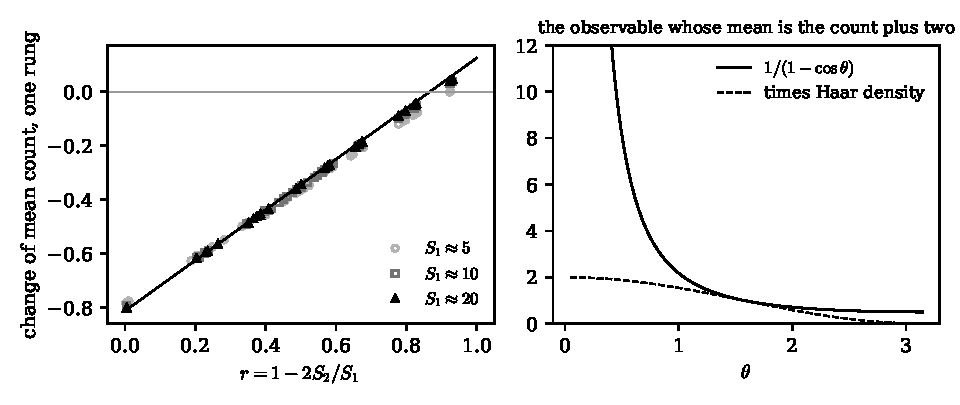
\includegraphics[width=\textwidth]{figures/firstrung.pdf}
\caption[The first rung theorem]{Left: the exact change of the mean count over one rung for $180$ random laws of the class $\mathcal L$ of three sizes, against the line $-\frac{13}{16}+\frac{15}{16}r$ of Theorem~\ref{thm:firstrung}. Right: the observable $1/(1-\cos\theta)$ of Proposition~\ref{prop:observable}, and its product with the Haar density, which is $1+\cos\theta$.}
\label{fig:firstrung}
\end{figure}

\paragraph{\normalfont\scshape On the lattice.} Proposition~\ref{prop:observable} makes sense for any law of a plaquette variable, whether or not it lies in $\mathcal M$: define the count of a lattice measure as $E[1/(1-\frac12\operatorname{tr}U_p)]-2$. It is finite on any finite lattice, since the density of a plaquette at the identity is bounded, it is $2\beta-\frac76$ for heat kernel plaquettes and $2\kappa-\frac32$ for Wilson plaquettes at weak coupling in two dimensions, where the plaquettes are independent, and it is zero for Haar measure. It is a candidate for the quantity to follow under blocking on $\mathbb Z^4$, in place of the coupling, with the advantage that it is defined without reference to an action. The next section computes it on a four dimensional lattice.

So two of the three numbers are theorems, for the first rung, and the third, $-\frac12$ from heat kernels, is a theorem once $r\to\frac13$ is proved. The proof does not go beyond it, because decimation is not known to keep a law in $\mathcal L$: that is Conjecture~\ref{conj:Lclosed}. If the conjecture holds, the theorem applies at every rung for as long as the count is large; if in addition the variance recursion of Section~\ref{sec:hypergeometric}, which is a leading order derivation, holds with a remainder, the ratio follows $r'=\frac5{16}+\frac1{16}r$ to its fixed point $\frac13$, and the drift settles at $-\frac12$ per rung from any start in $\mathcal L$; that is the constant drift seen in the exact ladder above and the reason the Wilson law, after one rung of gain, loses count like a heat kernel. Table~\ref{tab:firstrung} compares the theorem with exact rungs.

\begin{table}[t]
\centering\small
\begin{tabular}{lcccc}
\toprule
law in $\mathcal L$ & count & $r$ & exact & theorem \\ \midrule
$40$ zeros at $\gamma=1$ & $40.00$ & $0$ & $-0.805$ & $-0.813$ \\
$60$ zeros at $\gamma=2$ & $39.51$ & $0.333$ & $-0.499$ & $-0.500$ \\
$80$ random zeros drawn uniformly from $[1,6]$ & $38.08$ & $0.457$ & $-0.388$ & $-0.384$ \\
$120$ zeros at $\gamma=5$ & $39.01$ & $0.667$ & $-0.193$ & $-0.188$ \\
$300$ zeros at $\gamma=20$ & $27.24$ & $0.905$ & $+0.021$ & $+0.036$ \\
\bottomrule
\end{tabular}
\caption[The first rung against the theorem]{The change of the mean count over one exact rung from laws of the class $\mathcal L$, against $-\frac{13}{16}+\frac{15}{16}r$. The mean count agrees with $E[1/(1-\cos\theta)]-2$ computed by quadrature to all digits shown.}
\label{tab:firstrung}
\end{table}

\section{The count on a four dimensional lattice}\label{sec:countlattice}\index{mean count!on the lattice}\index{link integration}

The plain average of $1/(1-\frac12\operatorname{tr}U_p)$ over a simulation has a finite mean and an infinite variance, because the density of a plaquette at the identity is positive and the Haar weight vanishes there only like $\theta^2$. One link integration removes the difficulty.

\begin{proposition}[an estimator with finite variance]\label{prop:linkint}
Let $W$ be a random element of SU(2) with class density $\sum_nn\,u_n\chi_n$, where $\sum_nn\,u_n<\infty$, and $Y$ a fixed element. Then
\[
E\Big[\frac{1}{1-\frac12\operatorname{tr}(WY)}\Big]=2\sum_{n\ge1}u_n\,\chi_n(Y).
\]
In a lattice gauge theory with Wilson action, a link given all the others is $WV^{-1}$ with $V$ the normalised sum of its staples and $u_n=I_n(\kappa)/I_1(\kappa)$, $\kappa=\beta|{\rm staples}|$ with $|{\rm staples}|$ the norm of the staple sum. So for any loop that passes once through the link, with $R$ the rest of the loop, the count of the loop is the average of $2\sum_n\big(I_n(\kappa)/I_1(\kappa)\big)\chi_n(V^{-1}R)-2$, a bounded function of the configuration.
\end{proposition}

\begin{proof}
$\int\chi_n/(1-\cos\theta)$ against Haar measure is $\frac2\pi\int_0^\pi\chi_n(\theta)(1+\cos\theta)\,d\theta=2$ for every $n$, so $1/(1-\cos\theta)=2\sum_n\chi_n$ as a distribution on class functions, and $E\,\chi_n(WY)=u_n\chi_n(Y)$ for a conjugation invariant $W$.
\end{proof}

We ran it on an $8^4$ lattice, forty configurations at each coupling, for the plaquette and for the $2\times2$ loop. Beside each count we put the count of a Wilson law and of a heat kernel with the same fundamental coefficient $u_2=\langle\frac12\operatorname{tr}\rangle$: by Lemma~\ref{lem:Lcount} the two differ through the ratio $r$, so the comparison says which shape the lattice law has.

\begin{table}[t]
\centering\small
\begin{tabular}{rcccccc}
\toprule
 & \multicolumn{3}{c}{plaquette} & \multicolumn{3}{c}{$2\times2$ loop} \\
$\beta$ & count & Wilson & heat & count & Wilson & heat \\ \midrule
$1.5$ & $2.173(4)$ & $2.172$ & $1.901$ & $0.071(2)$ & $0.077$ & $0.075$ \\
$2.0$ & $3.666(6)$ & $3.686$ & $3.252$ & $0.302(3)$ & $0.316$ & $0.299$ \\
$2.3$ & $5.234(11)$ & $5.348$ & $4.809$ & $0.794(6)$ & $0.866$ & $0.781$ \\
$2.5$ & $6.299(11)$ & $6.477$ & $5.896$ & $1.227(6)$ & $1.364$ & $1.207$ \\
$2.7$ & $7.193(7)$ & $7.403$ & $6.801$ & $1.557(4)$ & $1.756$ & $1.542$ \\
$3.0$ & $8.496(13)$ & $8.731$ & $8.108$ & $2.038(7)$ & $2.312$ & $2.023$ \\
$4.0$ & $12.636(11)$ & $12.915$ & $12.267$ & $3.567(8)$ & $4.004$ & $3.545$ \\
\bottomrule
\end{tabular}
\caption[The count on an $8^4$ lattice]{The count $E[1/(1-\frac12\operatorname{tr}U)]-2$ of the plaquette and of the $2\times2$ loop in SU(2) lattice gauge theory on $8^4$, by the estimator of Proposition~\ref{prop:linkint}, with the counts of the Wilson law and of the heat kernel having the same $\langle\frac12\operatorname{tr}U\rangle$. Errors are standard errors over forty configurations and ignore autocorrelation.}
\label{tab:countlattice}
\end{table}

Two things can be read from Table~\ref{tab:countlattice}. The plaquette of the four dimensional theory has, at strong coupling, the count of a Wilson law to the accuracy measured, and moves a third of the way toward the heat kernel by $\beta=2.5$: the interaction with its neighbours gives the one plaquette law some of the curvature that the Wilson action lacks. And the $2\times2$ loop has the count of a heat kernel to within two per cent from $\beta=2$ on, and not that of a Wilson law, from which it differs by five to twelve per cent: a holonomy that is a product of several fluctuating pieces has the shape of a heat kernel. This is what the ladder does to a Wilson law in one decimation, and what the first rung theorem measures through $r$; here it is seen in the full theory.

\begin{figure}[t]
\centering
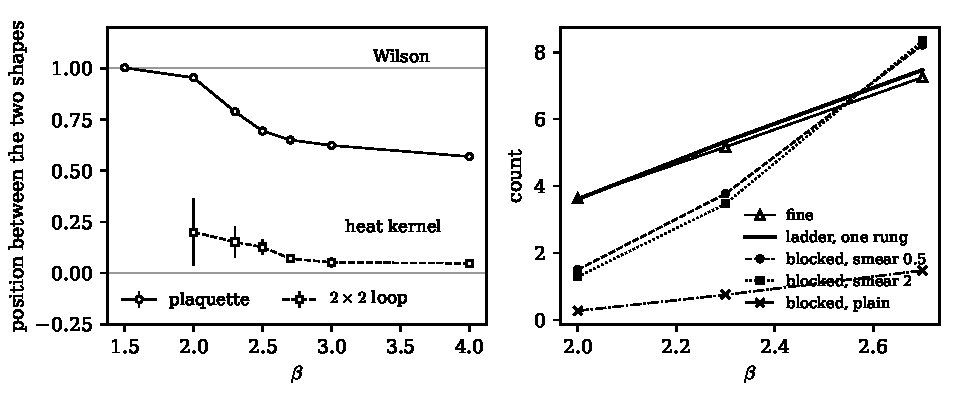
\includegraphics[width=\textwidth]{figures/count_lattice.pdf}
\caption[Shapes and counts on the lattice]{Left: the position of the measured count between that of the heat kernel, at $0$, and that of the Wilson law, at $1$, with the same $u_2$, for the plaquette and the $2\times2$ loop on $8^4$. Right: the count of the fine plaquette, of one rung of the ladder, and of the blocked plaquette for three blockings.}
\label{fig:countlattice}
\end{figure}

For a blocked lattice no link can be integrated out once the blocked links are smeared, and we took the count from the characters, $2\sum_{n\le40}E\chi_n-2$, each term of which has finite variance; on the unblocked lattice this agrees with the table to about two standard errors. Table~\ref{tab:countblocked} sets the count of the blocked plaquette, for two amounts of smearing, beside one exact rung of the ladder started from the Wilson law matched to the fine plaquette.

\begin{table}[t]
\centering\small
\begin{tabular}{rccccc}
\toprule
$\beta$ & fine & ladder & blocked, plain & smear $0.5$ & smear $2$ \\ \midrule
$2.0$ & $3.64(2)$ & $3.61$ & $0.27(4)$ & $1.50(3)$ & $1.29(7)$ \\
$2.3$ & $5.17(3)$ & $5.33$ & $0.75(6)$ & $3.77(9)$ & $3.47(12)$ \\
$2.7$ & $7.25(8)$ & $7.47$ & $1.48(3)$ & $8.22(11)$ & $8.34(23)$ \\
\bottomrule
\end{tabular}
\caption[The count under blocking, lattice against ladder]{The count of the plaquette on $8^4$, the count after one exact rung of the ladder from the matched Wilson law, and the count of the plaquette of the lattice blocked to $4^4$ with scale factor two: blocked links without smearing, and with the staples added with weight $0.5$ and $2$ before projection.}
\label{tab:countblocked}
\end{table}

At $\beta=2.0$ and $2.3$ the blocked lattice has a smaller count than the ladder, for every smearing: the true flow loses order faster than the ladder does, which is the direction of the comparison asked for in Chapter~\ref{ch:sandwich}, since the count is the mean of an increasing function of $\cos\theta$. At $\beta=2.7$ the inequality is reversed for the smeared blockings. The smeared blocked plaquettes have the count of a Wilson law with their $u_2$, within errors, and the unsmeared ones are close to that of a heat kernel, so the shape of the blocked law depends on the blocking as much as its coupling does.

To see whether the reversal at $\beta=2.7$ is an effect of the small box we repeated the computation on $16^4$, with two blockings, to $8^4$ and to $4^4$, smearing $0.5$, thirty configurations at each coupling.

\begin{table}[t]
\centering\small
\begin{tabular}{rcccccc}
\toprule
 & \multicolumn{2}{c}{fine} & \multicolumn{2}{c}{blocked once} & \multicolumn{2}{c}{blocked twice} \\
$\beta$ & lattice & ladder & lattice & ladder & lattice & ladder \\ \midrule
$2.3$ & $5.23(1)$ & $5.34$ & $3.77(4)$ & $5.34$ & $1.27(8)$ & $4.87$ \\
$2.5$ & $6.31(1)$ & $6.48$ & $6.09(2)$ & $6.51$ & $4.04(16)$ & $6.04$ \\
$2.7$ & $7.22(1)$ & $7.43$ & $8.14(7)$ & $7.48$ & $6.75(17)$ & $7.01$ \\
\bottomrule
\end{tabular}
\caption[Two blockings on $16^4$]{The count of the plaquette on $16^4$ and after one and two blockings with scale factor two and smearing $0.5$, against the count after the same number of exact rungs of the ladder from the Wilson law matched to the fine plaquette.}
\label{tab:countblocked2}
\end{table}

The reversal is not an effect of the box: at $\beta=2.7$ the plaquette blocked once has a larger count than the fine one on $16^4$ also, $8.14$ against $7.22$, and exceeds the ladder. It is an effect of the smearing, which at weak coupling removes short distance fluctuations from the blocked link faster than a rung of the ladder does. After the second blocking the lattice is below the ladder at all three couplings, and at $\beta=2.3$ and $2.5$ it is below at both levels, by a margin that grows with the level. So the comparison holds where the coupling has begun to run and fails, for this blocking, at the first step from weak coupling: an inequality between the two flows has to be asked either with an error term or from the second step on, and it depends on the blocking. These are small lattices and a count that depends on the choice of blocked link; they are an illustration of how the observable behaves, not a measurement of the flow.

\paragraph{\normalfont\scshape Log concavity.} One half of Open problem~\ref{op:logconcave} has a short answer.

\begin{proposition}\label{prop:Llogconcave}
For every law of the class $\mathcal L$ the count law $\pi$ is log concave.
\end{proposition}

\begin{proof}
For a finite product the unnormalised weights $\nu_0$ are those of a sum of $N$ independent Bernoulli variables, so by Newton's inequalities $\nu_0(j)^2\ge(1+1/j)\,\nu_0(j-1)\,\nu_0(j+1)$. The count law is $\pi(j)\propto\nu_0(j)Z_j$ with $Z_j=C_{j+1}/2^j$, and from $C_{n+1}/C_n=2(2n+1)/(n+2)$,
\[
\frac{Z_{j+1}Z_{j-1}}{Z_j^2}=1+\frac{3}{2j^2+7j+3}\le1+\frac1j .
\]
Infinite products follow in the limit.
\end{proof}

For the other half, whether coalescence preserves log concavity, we have only evidence: in rational arithmetic, over $400$ random log concave $\nu_0$ and $400$ random log concave $\pi$ on up to fifteen points, one coalescence left the law log concave every time, with smallest ratios $\nu(j)^2/\nu(j-1)\nu(j+1)$ of $1.049$ and $1.223$.

\section{What is proved and what is left}

Proved:
\begin{itemize}
\item the exact ladder lives in $\mathcal M$; bond moving is addition of counts, and decimation is a coalescence with the hypergeometric kernel of Theorem~\ref{thm:hypergeometric}, which is totally positive of order two;
\item the mean count is the observable $E[1/(1-\cos\theta)]-2$ (Proposition~\ref{prop:observable}), with an estimator of finite variance on the lattice (Proposition~\ref{prop:linkint});
\item under convolution the mean count obeys the harmonic law with an error $O(1/J)$ (Theorem~\ref{thm:harmonic});
\item from any law with real zeros the first rung changes the mean count by $-\frac{13}{16}+\frac{15}{16}r+o(1)$ (Theorem~\ref{thm:firstrung});
\item every law with real zeros has a log concave count (Proposition~\ref{prop:Llogconcave}).
\end{itemize}

Not proved, and now sharply posed:

\begin{problem}\label{op:Qtp2}
Show that $Q(j\mid a,b)$ is totally positive of order two in $(j,a)$ for every $b$. (Solved: Corollary~\ref{cor:hypergeometric}.)
\end{problem}

\begin{problem}\label{op:logconcave}
Show that the exact ladder preserves log concavity of $\nu_0$. Sums of independent log concave counts are log concave; the question is the coalescence. (Proposition~\ref{prop:Llogconcave} shows that every law of the class $\mathcal L$ has a log concave count; exact computation supports the rest.)
\end{problem}

\begin{problem}\label{op:drift}
Explain the constant drift. (Answered to leading order in Section~\ref{sec:hypergeometric}: the drift is $-\frac{13}{16}+\frac{15}{16}r$ and $r\to\frac13$. Theorem~\ref{thm:firstrung} proves the drift formula for the first rung from any law of the class $\mathcal L$, but $r\to\frac13$ for heat kernels is not proved; later rungs wait on Conjecture~\ref{conj:Lclosed}.)
\end{problem}

These would be steps toward a contraction theorem for the exact ladder, but they are not sufficient and the target needs care. Section~\ref{ch:kingman} shows that the ladder is not monotone on all of $\mathcal M$, nor on all laws with log concave count, and that from a Wilson law with $\kappa\ge2$ the fundamental coefficient rises at the first rung. The theorem to aim for concerns the orbit of a heat kernel, or a class of laws that contains it and is preserved, and that class is not yet identified. What the count formulation does remove is the bad cap at the antipode: on the group every $f_j$ with $j\ge1$ vanishes there, and on the integers only the state $j=0$ charges it.

\section{The same theorem for the circle}

It is worth seeing how much of this is special to SU(2). On U(1) the analogous densities are $(1+\cos\theta)^j$ with respect to Lebesgue measure on the circle, with Fourier coefficients $\binom{2j}{j-n}/\binom{2j}{j}$: the walk again, now without the factor $(J+1)/J$ and with the node $n=0$ included. The proof of Theorem~\ref{thm:coalescence} goes through word for word with nodes $0,1,4,\dots,a^2$, since it used only the complete monotonicity of $w_N$. So the family of mixtures of $(1+\cos\theta)^j$ on the circle is closed under convolution with a positive kernel as well, and the Villain and Wilson laws of the abelian theory lie in it (for the Villain law this is the circle analogue of Theorem~\ref{thm:kingman}, with death rate $\frac12j^2$). What differs is the mean: on the circle the functional $\mathsf W$ is not available, and the abelian ladder has the exponentially small decrement found for U(1) in Chapter~\ref{ch:path}, not a constant one. The positivity is common to both groups; the drift of one half is the nonabelian curvature.

\section{Assessment}

This is the first statement in the book about the exact ladder that is a theorem at every coupling and uses no projection. It does not touch $\mathbb Z^4$. Its use for the real problem is indirect and we state it as a hope: the family $\mathcal M$ is defined on one link, and the Wilson measure on any lattice is a product of members of $\mathcal M$ over plaquettes; so the lattice measure has a representation by integer counts on plaquettes with positive weights before the links are integrated. Whether blocking on $\mathbb Z^4$ acts on those counts by a positive kernel, as it does on a hierarchical lattice, is the comparison problem of Chapter~\ref{ch:sandwich} in its most concrete form so far.

\section{Kingman's coalescent in the heat kernel}\label{ch:kingman}\index{Kingman, J. F. C.}\index{coalescent}\index{Wright Fisher diffusion}\index{Ewens sampling formula}\index{duality}

The count of the preceding sections was found by multiplying out a product. It has a name. In the variable $y=\cos^2(\theta/2)$ Brownian motion on SU(2) is a Wright Fisher diffusion, and the latent count is the number of ancestral lineages in Kingman's coalescent. The next sections prove that, draw three consequences, and then ask what else in Kingman's work, and in our book on statistical methods for genetics~\cite{Po26g}, bears on the gap. Of that book we use its contents; of Kingman, the papers of 1963, 1973 and 1982 \cite{Ki63,Ki73,Ki82}, and for the paintbox representation his paper of 1978.

\section{Brownian motion on SU(2) is a Wright Fisher diffusion}\label{sec:wf}

\begin{proposition}\label{prop:wf}
Let $y=\cos^2(\theta/2)=\frac12(1+\cos\theta)$. On class functions,
\[
\Delta=y(1-y)\,\partial_y^2+\big(\tfrac32-3y\big)\,\partial_y=2\,\mathcal G,
\]
where
\[
\mathcal G=\tfrac12y(1-y)\,\partial_y^2+\tfrac12\big(\theta_{\mathrm m,1}(1-y)-\theta_{\mathrm m,2}y\big)\partial_y,\qquad\theta_{\mathrm m,1}=\theta_{\mathrm m,2}=\tfrac32 .
\]
So the class angle of the Brownian motion with heat kernel $K_t$ is, in the variable $y$, the neutral two allele Wright Fisher diffusion with symmetric mutation and total mutation parameter $\theta_{\mathrm m}=3$, run for the time $\tau=t/2$ and started from fixation, $y=1$. Its stationary law is Beta with parameters $\frac32,\frac32$, which is Haar measure.
\end{proposition}

\begin{proof}
From $\Delta=\partial_\theta^2+2\cot\theta\,\partial_\theta$, $dy/d\theta=-\frac12\sin\theta$ and $\sin^2\theta=4y(1-y)$. The heat kernel has generator $\frac14\Delta=\frac12\mathcal G$.
\end{proof}

The identification is of the kind that Kac would have liked: the gene frequency of population genetics and the plaquette variable of gauge theory obey the same equation, with the dimension of the group, three, as the mutation rate.

\section{Duality: heat flow is the death of lineages}\label{sec:duality}

Let $A$ be the pure death process on the nonnegative integers that jumps from $m$ to $m-1$ at rate $\frac12m(m+2)$. For $\theta_{\mathrm m}=3$ this is the process counting the lineages of Kingman's coalescent in which each pair merges at rate one and each lineage is lost by mutation at rate $\theta_{\mathrm m}/2$: the rate is $\binom m2+\frac{3m}2=\frac12m(m+2)$. It comes down from infinity, and we write $P_\infty$ for its law started there.

\begin{theorem}[coalescent duality]\label{thm:kingman}
With $f_j\propto(1+\cos\theta)^j$ the densities of Theorem~\ref{thm:coalescence}:
\begin{enumerate}
\item[(i)] $f_a*K_s=\sum_{j\le a}P_a\big(A(s/2)=j\big)\,f_j$ for every $a\ge0$ and $s>0$;
\item[(ii)] $K_t=\sum_{j\ge0}P_\infty\big(A(t/2)=j\big)\,f_j$.
\end{enumerate}
The latent count of the heat kernel in Proposition~\ref{prop:latentcount} is the number of lineages of Kingman's coalescent with mutation, at time $t/2$.
\end{theorem}

\begin{proof}
By Lemma~\ref{lem:fjchar}, $f_j$ has coefficients $u_n(J)$ with $J=j+1$, and $u_n(J-1)/u_n(J)=(J^2-n^2)/(J^2-1)$. The death rate from $j$ is $\frac12j(j+2)=\frac12(J^2-1)$, so the generator $G$ of $A$ applied to $j\mapsto u_n(j+1)$ gives
\[
\tfrac12(J^2-1)\big[u_n(J-1)-u_n(J)\big]=-\tfrac12(n^2-1)\,u_n(J).
\]
Thus $j\mapsto u_n(j+1)$ is an eigenfunction of $G$ with eigenvalue $-\frac12(n^2-1)$, and $\E_a\big[u_n(A(\tau)+1)\big]=e^{-(n^2-1)\tau/2}u_n(a+1)$. With $\tau=s/2$ the right side is the $n$th coefficient of $f_a*K_s$, which is (i). As $a\to\infty$, $u_n(a+1)\to1$ for each $n$, $f_a$ tends to the unit mass at the identity, and (ii) follows.
\end{proof}

The proof is three lines because the work was done by Lemma~\ref{lem:fjchar}. In population genetics (ii) is the expansion of the transition density of the Wright Fisher diffusion in Beta laws weighted by the ancestral process, due to Griffiths~\cite{Gri80} and to Tavar\'e~\cite{Tav84}, and (i) is the statement that mixtures of Beta laws are preserved by the diffusion, with the death process moving the weights, which is the basis of the exact filters of Chaleyat Maurel and Genon Catalot~\cite{CMGC09} and of Papaspiliopoulos and Ruggiero~\cite{PR14}. The script \texttt{kingman\_dual.py} checks both: the count law from the product formula and Tavar\'e's series for the entrance law agree to $10^{-13}$ at $t=0.5$, $1$ and $2$, and the characters of $f_a*K_s$ computed from the matrix exponential of $G$ agree to $10^{-14}$.

\begin{figure}[t]
\centering
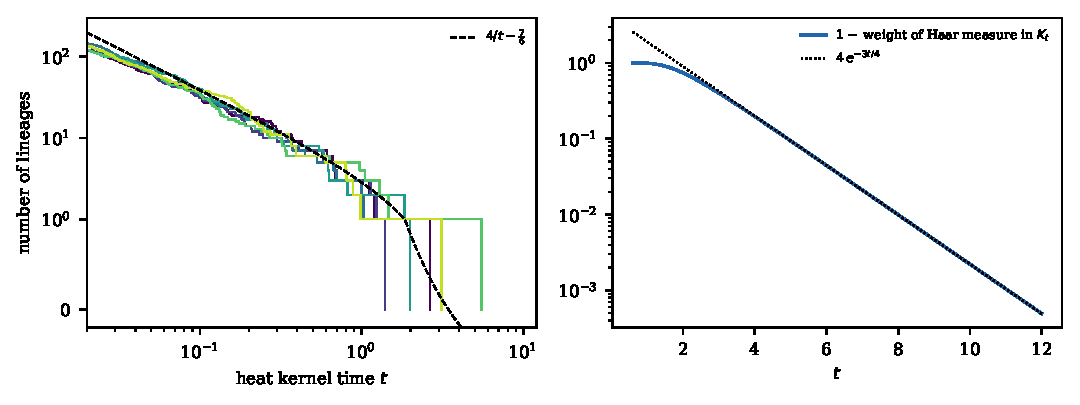
\includegraphics[width=\textwidth]{figures/kingman_fig.pdf}
\caption[Kingman's coalescent in the heat kernel]{Left: six paths of the death process with rates $\frac12m(m+2)$ started from $400$ lineages, against the heat kernel time $t=2\tau$, with the mean $4/t-\frac76$ of the entrance law. Right: one minus the weight of Haar measure in $K_t$, the probability that a lineage survives, with its asymptote $4e^{-3t/4}$; the rate is the gap.}
\label{fig:kingman}
\end{figure}

\section{Three consequences}

\paragraph{\normalfont\scshape A second proof of the likelihood ratio property.} Transition functions of birth and death processes are totally positive, by the theorem of Karlin and McGregor on coincidence probabilities~\cite{KM59}. Start $A$ from $N$. For $s>0$ the law $\delta_NP_s$ is below $\delta_N$ in the likelihood ratio order, as every law on $\{0,\dots,N\}$ is; applying the totally positive kernel $P_t$ preserves the order, so $\delta_NP_{t+s}$ is below $\delta_NP_t$. Let $N\to\infty$: the count of $K_{t+s}$ is below the count of $K_t$. Since $(1+x)^j$ is totally positive in $(j,x)$, the mixtures inherit the order, and $K_t/K_{t+s}$ is increasing in $\cos\theta$. This is Corollary~\ref{cor:mlrall}, with no product formula and no Laguerre: the likelihood ratio property of the heat kernel on SU(2) is the total positivity of Kingman's death process.

\paragraph{\normalfont\scshape The spectral gap is the death of the last lineage.} The time for $A$ to fall from infinity to $m$ is a sum of independent exponential variables with rates $\frac12k(k+2)$, $k>m$: a generalized gamma convolution whose Thorin measure sits on the Casimir values. In particular the weight of Haar measure in the heat kernel is a distribution function,
\[
P_\infty\big(A(t/2)=0\big)=P\Big(\sum_{k\ge1}\frac{2E_k}{k(k+2)}\le\frac t2\Big),
\]
with $E_k$ independent standard exponentials, and the slowest rate, $k=1$, is $\frac32$ in the time $\tau$, which is $\frac34$ in $t$: the spectral gap of the heat semigroup on SU(2), not the mass gap. The heat kernel has become Haar measure exactly when the last lineage has died. This is the cleanest instance in the book of its opening theme: a spectral gap is the lowest atom of a Thorin measure, and here the Thorin measure is that of an extinction time.

\paragraph{\normalfont\scshape The projected ladder is a computable filter.} In counts, the prediction step of the projected ladder is the death process run for a time, and the update step, bond moving, is the addition of independent counts. This is the structure of the exact filter for a Wright Fisher signal: observations add to the count, time removes from it, and the filter never leaves the mixtures of Beta laws. The difference is that the ladder observes itself. The filtering reading of Section~\ref{ch:spdefilter} is thus exact for the prediction and update steps in counts; the projection onto heat kernels is not part of that exactness.

\section{What Kingman's process does not explain}

Decimation in the exact ladder is the convolution of a law with itself, not with a heat kernel, and its kernel $Q(\cdot\mid a,b)$ of Theorem~\ref{thm:coalescence} is not a transition function of $A$. The kernel $Q$ has a genealogical reading: $Q(\cdot\mid a,b)$ is the hypergeometric law of the number of elements common to two random samples of sizes $a$ and $b$ from a population of $a+b+2$ (Theorem~\ref{thm:hypergeometric}).

Nor does duality make the ladder a contraction on all of $\mathcal M$, which it is not. Table~\ref{tab:notmonotone} records one exact rung, $k=4$ and $\ell^2=4$, from several starting laws.

\begin{table}[t]
\centering\small
\begin{tabular}{lccc}
\toprule
starting law & count & change & change of $u_2$ \\ \midrule
heat kernel, $\beta=4$ & 6.87 & $-0.507$ & $-0.017$ \\
$f_5$, a point mass at $5$ & 5.00 & $-0.754$ & \\
Wilson, $\kappa=1$ & 1.24 & $-0.405$ & $-0.053$ \\
Wilson, $\kappa=4$ & 6.63 & $+0.034$ & $+0.021$ \\
Wilson, $\kappa=16$ & 30.5 & $+0.110$ & $+0.002$ \\
half Haar, half $f_{20}$ & 10.0 & $+8.37$ & \\
geometric count, ratio $0.9$ & 8.99 & $+6.50$ & \\
\bottomrule
\end{tabular}
\caption[One exact rung from several starting laws]{The mean count, its change, and the change of the fundamental coefficient over one exact rung of the ladder, from several starting laws in $\mathcal M$. From heat kernels the mean count and the fundamental coefficient fall. From Wilson laws at $\kappa=4$ and $16$ the fundamental coefficient rises at the first rung, and from bimodal laws the count rises sharply. The geometric count is truncated at $100$.}
\label{tab:notmonotone}
\end{table}

Two lessons. A law with two components, one near Haar measure and one concentrated, becomes more ordered under a rung, because raising a density to a power favours its peak; so no functional is monotone on all of $\mathcal M$, and any theorem must be about a class of laws. And the Wilson law at $\kappa\ge2$ gains order at its first rung: bond moving of a Wilson law is exact, $\kappa\mapsto k\kappa$, with none of the curvature loss of Theorem~\ref{thm:scaledmlr}, and the loss appears only once the law has taken the shape of a heat kernel. The inequality $R(\beta)<\beta$ is a statement about the ladder in heat kernel coordinates, as it was stated, and not about one rung from an arbitrary start. We tested two candidate classes on three thousand random laws: when $\nu_0$ is log concave the fundamental coefficient can still rise, by up to $0.03$, and the same is true for sums of independent Bernoulli counts such as a binomial with mean $2$. The orbit of a heat kernel is monotone at every rung we computed. The drift law of Section~\ref{sec:hypergeometric} explains the table to leading order, apart from the Wilson $\kappa=1$ row (count $1.24$, too small for an asymptotic formula) and the geometric row (predicted $+8.56$ against $+6.50$): the change of the mean count is $-\frac{13}{16}+\frac{15}{16}r$ with $r$ the ratio of variance to mean of the count, which is $0$ for a point mass, $\frac13$ for a heat kernel and $1$ for a Wilson law, and $r$ relaxes to $\frac13$ in one or two rungs.

\section{Kingman's other tools}

\paragraph{\normalfont\scshape Random walks with spherical symmetry.} Kingman's paper of 1963~\cite{Ki63} studied the addition of independent random vectors through their lengths alone, and found that the lengths compose by a convolution of their own, indexed by the dimension, with Bessel functions as characters. Convolution of class functions on SU(2) is the compact member of that family: the radial parts of products of independent group elements compose by the Gegenbauer convolution on $[-1,1]$, with the $\chi_n/n$ as characters. Theorem~\ref{thm:coalescence} is a positivity theorem for that convolution on the cone spanned by the powers of $1+x$. Kingman's flat case is the limit of large counts, where $ab/(a+b+2)$ becomes the harmonic rule for precisions.

\paragraph{\normalfont\scshape The subadditive ergodic theorem.} Kingman's theorem~\cite{Ki73} gives the existence of the limit of $\frac1n\log\|X_n\cdots X_1\|$ for stationary products, and with it Lyapunov exponents. Two uses here. The existence of the string tension on the hierarchical lattice in Chapter~\ref{ch:progress} is a deterministic argument of telescoping type, a relative of subadditivity. And the stochastic ladder suggested, and not pursued, in Section~\ref{ch:spdefilter}, a ladder with a common noise at each rung, would have a string tension that is a Lyapunov exponent in Kingman's sense, which exists if the hypotheses of his theorem hold; its positivity is the open question.

\paragraph{\normalfont\scshape Exchangeable partitions.} Kingman's representation of exchangeable partitions through paintbox processes (his paper of 1978) is de Finetti's theorem for partitions, and the Ewens sampling formula~\cite{Ew72} is its best known case. It joins the exchangeability of Chapter~\ref{ch:hitting} to the structure of the ladder.

\section{The genetics volume}

Our \emph{On Statistical Methods for Genetics: Fisher, Ewens and the Bayesian Programme}~\cite{Po26g} treats population genetics as statistical inference. Four of its themes recur here.

\begin{center}
\small
\begin{tabular}{p{0.44\textwidth}p{0.48\textwidth}}
\toprule
genetics volume & this book \\ \midrule
the number of alleles in a sample is a sum of independent Bernoulli variables, and is sufficient for the mutation rate under the Ewens formula & the count $M_0$ of the heat kernel (Proposition~\ref{prop:latentcount}, before reweighting) is a sum of independent Bernoulli variables with parameters $1/\gamma_m$; the action is sufficient for the coupling \\
the Ewens formula from de Finetti's theorem & plaquettes exchangeable under a prior on the coupling; mixtures and their large deviations \\
the number of segregating sites is not sufficient; pooled encoders see only the site frequency spectrum & pooled characters; an attention head finds the sufficient coordinate among eight \\
learned quantile maps for the coalescent attain the Bayes risk & GBC generators for the coupling and for the gap \\
\bottomrule
\end{tabular}
\end{center}

The first row is more than a parallel. In the Ewens formula with parameter $\theta_{\mathrm m}$ the number of alleles among $n$ genes is $\sum_i\xi_i$ with $\xi_i$ Bernoulli of parameter $\theta_{\mathrm m}/(\theta_{\mathrm m}+i-1)$. In the heat kernel the count is $\sum_m\xi_m$ with parameter $1/\gamma_m(t)$. Both are P\'olya frequency laws and the number of alleles is sufficient for $\theta_{\mathrm m}$, as the action is for the coupling. The roots $\gamma_m(t)$ of Theorem~\ref{thm:product} are in this sense the allele probabilities of the heat kernel. The parallel is of the sums, not of the coalescents: the Ewens count is the number of lineages lost to mutation going back in time, while the sum $M_0$ is not the number of lineages that survive to time $t/2$. That number is the latent count $A(t/2)$ of Theorem~\ref{thm:kingman}, whose law is that of $M_0$ reweighted by $C_{m+1}2^{-m}$ (Lemma~\ref{lem:Lcount} and Proposition~\ref{prop:latentcount}).

\section{Are these ideas useful?}

Yes, and more directly than any other neighbour of the ladder. Kingman's coalescent is not an analogy for the ladder on counts; it is the linear half of it. The duality gives a three line proof that heat kernels lie in $\mathcal M$, a second proof of the likelihood ratio property from total positivity of a death process, an identification of the spectral gap of the heat semigroup with the extinction of the last lineage, and the exact filter structure of the projected ladder. What it does not give is the nonlinear half, the self convolution of the exact ladder, and it does not reach $\mathbb Z^4$.

The question it suggests is the right one to end on. Population genetics has a second classical object beside the coalescent: the ancestral graph with selection and recombination, in which lineages branch as well as merge. Bond moving is a branching, by the factor $k$; decimation is a merging. The exact ladder is a branching and coalescing system of lineages, of the kind studied for the ancestral selection graph of Krone and Neuhauser~\cite{KN97}, and its extinction is confinement. Whether the methods that give extinction criteria for such graphs apply here is, as far as we know, an open and well posed question.

\section*{Exercises}
\begin{enumerate}
\item (Section~\ref{sec:hypergeometric}) Verify Lemma~\ref{lem:fjchar} for $j=2$ by expanding $(1+x)^2$ in $\chi_1,\chi_2,\chi_3$.
\item (Section~\ref{sec:hypergeometric}) Compute $Q(\cdot\mid2,3)$ from the Newton formula in the proof and compare with $\big(\frac27,\frac47,\frac17\big)$.
\item Show that $w_N$ is not completely monotone beyond $(N+1)^2$, and explain why the proof needs $\bar a\le\bar b$.
\item Prove that the mean count of the Wilson law is $\kappa$ before reweighting and find it after reweighting, using Corollary~\ref{cor:meancount}.
\item (Section~\ref{sec:wf}) Verify Proposition~\ref{prop:wf} and find the Wright Fisher diffusion that corresponds to the class functions of SU(2) acting on $S^2$ in place of $S^3$.
\item (Section~\ref{sec:duality}) Show from Theorem~\ref{thm:kingman} that the mean count of the heat kernel satisfies $m'(\tau)=-\frac12\E[A(A+2)]$ and deduce $m\approx2/\tau$ for small $\tau$.
\item (Section~\ref{sec:duality}) Compute $P_\infty(A(\tau)=0)$ to three figures at $t=1$ and $t=2$ from the sum of exponentials.
\item For which starting counts $a$ is the law of $A(\tau)$ under $P_a$ log concave for all $\tau$?
\item Find a two point law in $\mathcal M$ whose fundamental coefficient rises under one rung, and explain it by the peak of the bond moved density.
\end{enumerate}
